\documentclass[tikz,border=5pt]{standalone}
\usepackage{amsmath}
\usepackage{amssymb}
\usetikzlibrary{arrows.meta,positioning,calc,fit}
\usetikzlibrary{positioning,shapes.geometric}
\begin{document}
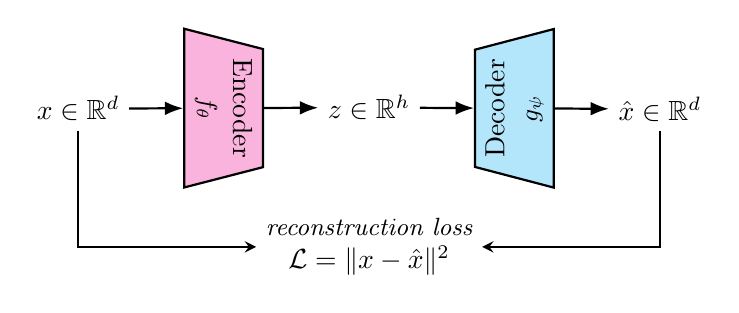
\begin{tikzpicture}[
    >=Latex,
    node distance=8mm and 12mm,
    small/.style={font=\itshape},
    trap/.style={
        draw, thick,
        trapezium,
        trapezium stretches=true,
        minimum width=19mm,
        minimum height=10mm,
        align=center
    },
]

\node (x) {$x\in\mathbb R^d$};

% Encoder: 左长右短（右边更“斜”进来） => 右角更小
\node[trap, right=of x,yshift=9mm,
      trapezium left angle=75,
      trapezium right angle=75,rotate=-90,fill=magenta!30] (enc)
      {Encoder\\\small $f_\theta$};

\node[right=of enc,yshift=9mm] (z) {$z\in\mathbb R^h$};

% Decoder: 左短右长（左边更“斜”进来） => 左角更小
\node[trap, right=of z,yshift=-9mm,
      trapezium left angle=75,
      trapezium right angle=75,rotate=90,fill=cyan!30] (dec)
      {Decoder\\\small $g_\psi$};

\node[right=of dec,yshift=-9mm] (xhat) {$\hat{x}\in\mathbb R^d$};
\draw[->, thick] (x) -- (enc);
\draw[->, thick] (enc) -- (z);
\draw[->, thick] (z) -- (dec);
\draw[->, thick] (dec) -- (xhat);

\node[below=10mm of z, align=center, small] (loss) {{\small reconstruction loss}\\$\mathcal L=\|x-\hat{x}\|^2$};
\draw[-stealth, thick] (xhat.south) |- (loss.east);
\draw[-stealth, thick] (x.south) |- (loss.west);

\end{tikzpicture}
\end{document}


